\documentclass{beamer}
\mode<presentation>{
	\usetheme{Madrid}
}
\usepackage{graphicx}
\usepackage{booktabs}
\usepackage{lmodern}
\usepackage{enumerate}
\usepackage{amsmath}
\usepackage{ragged2e}

\title[machine learning]{Machine Learning}
\author{Nguyen Quoc Huy}
\institute[NID]{
	Seoul National University of Science and Technology\\
	\medskip
	\textit{nqhuy2205@gmail.com}
}
\date{\today}
\begin{document}
\begin{frame}
\titlepage
\end{frame}

\begin{frame}
\frametitle{Contents}
\tableofcontents
\end{frame}

\section{Introduction to Machine learning}
\begin{frame}
\frametitle{What is machine learning}
Machine learning is the idea that there are generic algorithms that can tell you something interesting about a set of data without you having to write any custom code specific to the problem. Instead of writing code, you feed data to the generic algorithm and it builds its own logic based on the data.
\end{frame}

\begin{frame}
\frametitle{Machine Learning Techniques}
\begin{figure}
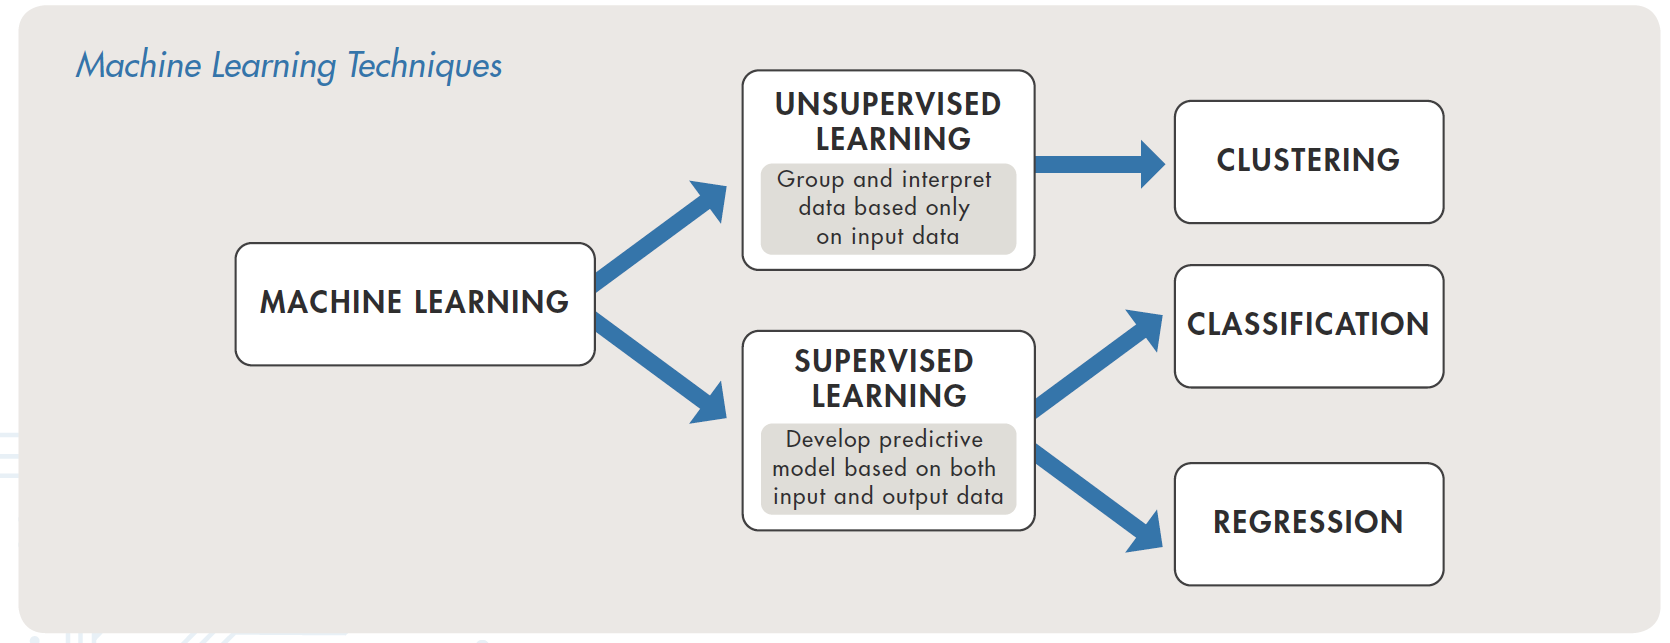
\includegraphics[scale=0.26]{figs/ml_techniques.PNG}
\end{figure}
\end{frame}

\begin{frame}
\frametitle{Machine Learning Model}
\begin{itemize}
	\item function h is called hypothesis
	\item hypothesis h: predict function
	\item hypothesis h: classifier
\end{itemize}
\begin{figure}
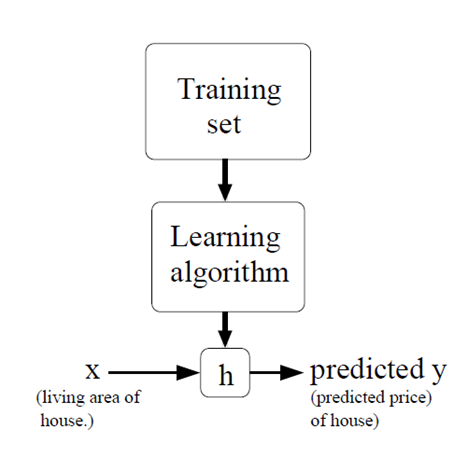
\includegraphics[scale=0.4]{figs/ml_model.png}
\end{figure}
\end{frame}

\begin{frame}
\frametitle{Machine Learning Algorithm}
\begin{figure}
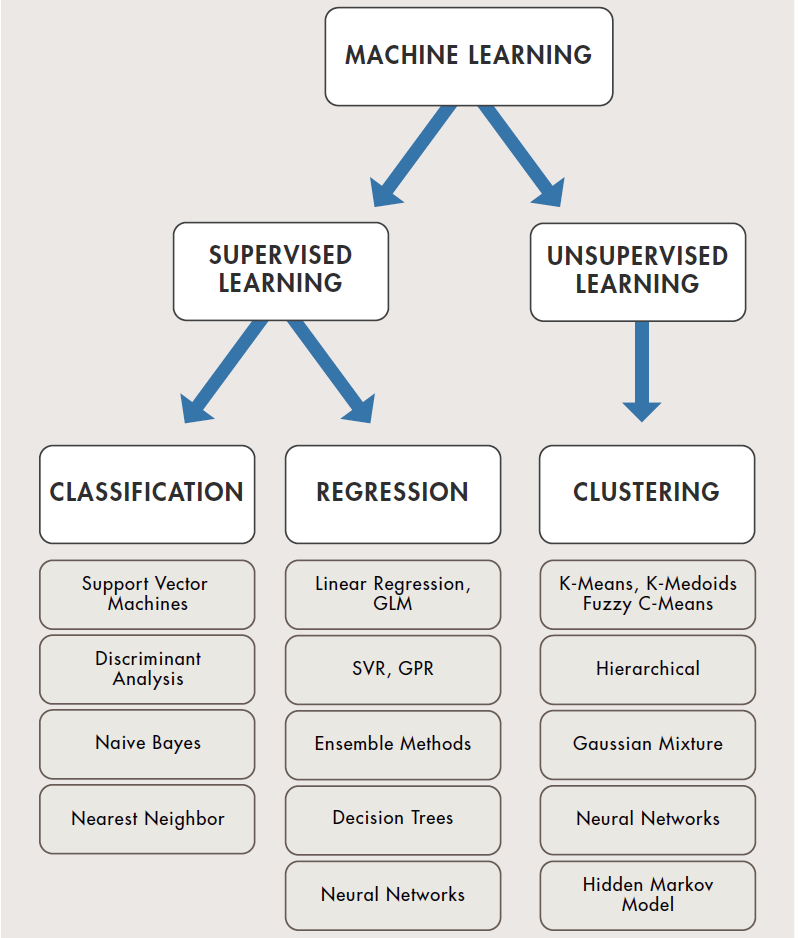
\includegraphics[scale=0.3]{figs/ml_algorithym.PNG}
\end{figure}
\end{frame}

\section{Regression}
\begin{frame}
\frametitle{Regresstion}
\begin{itemize}
	\item Linear Regression
	\begin{itemize}
		\item hyphothesis $h$ is a linear function
	\begin{equation}
		h_{\theta}(x) =\theta _{0} + \theta _{1}x_1+ \theta _{2}x_2
	\end{equation}
	\item $\theta _i$'s are called {\bf Weights}. Let $x_0 = 1$
	\begin{equation}
		h(x)=\sum_{i=0}^{n}\theta _{i}x_{i} = \theta ^{T}x
	\end{equation}
	\end{itemize}
	\item Logistic Regression
	\begin{itemize}
	\item hypothesis $h$ is a sigmoid function
	\begin{equation}
		h_{\theta}(x) = g(\theta ^{T}x) =\frac{1}{1 + e^{-\theta ^{T}x}}
	\end{equation}
	\end{itemize}
	\item Generalized Linear Models
\end{itemize}
\end{frame}

\begin{frame}
\frametitle{Linear Regression}
\begin{itemize}
	\item hyphothesis $h$
	\begin{equation}
		h_{\theta}(x) =\theta _{0} + \theta _{1}x_1+ \theta _{2}x_2
	\end{equation}
	\item Cost function (Lost function)
	\begin{itemize}
		\item $||h_{\theta}(x^{(i)})-y^{(i)}||$
		\item $J(\theta)=\frac{1}{2m}\sum_{i=1}^{m}(h_{\theta}(x_{(i)})-y^{(i)})^2$\\so we want $\theta=\arg\min(J(\theta))$
	\end{itemize}
	\item Gradient Descent
\end{itemize}
\end{frame}

\section{The {\it k}-means clustering}
\begin{frame}
\frametitle{The {\it k}-means clustering}
We are given a training set $ {\bf X} = [x^{(1)}, x^{(2)},..., x^{(N)}]$, and we want to group data into $K$ {\bf clusters}
\begin{figure}
	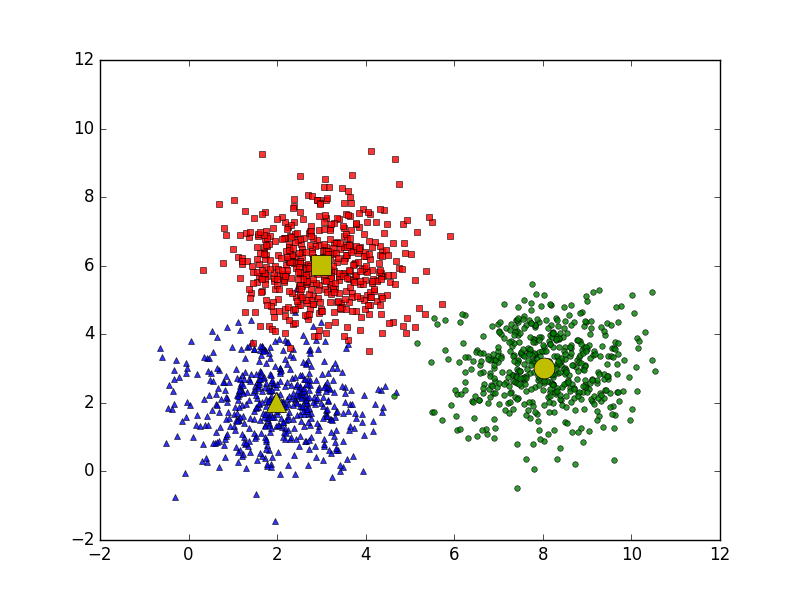
\includegraphics[scale=0.3]{figs/figure_2.png}
\end{figure}
\end{frame}



\begin{frame}
\frametitle{The {\it k}-means clustering: Describe label matrix}
% For each data point $x^{(i)}$, introduce a corresponding set of binary indicator variables $y^{(i)}_k \in \{0,1\}$, where $k = 1,...,K$ describing which of 
Introduce $y^{(i)} =[y_{1}^{(i)},y_{2}^{(i)},...,y_{K}^{(i)},]$ is the label vector of data point $x^{(i)}$ so that if data point $x^{(i)}$ is assigned to cluster $k$ then $y^{(i)}_k = 1$ and $y^{(i)}_j = 0$ for $j \neq k$
% $\forall x^{(i)} \in k^{th}$ cluster we have $y^{(i)}_k = 1$ and $y^{(i)}_j = 0, \forall j \neq k$\\
\begin{equation}
y^{(i)}_k \in \{0,1\}, \sum^K_{k=1}y^{(i)}_k = 1
\end{equation}
\quad Ex:\\
\qquad $x^{(1)}$ belong to $1^{st}$ cluster, $y^{(1)}=[1,0,0,...]$\\
\qquad $x^{(2)}$ belong to $2^{nd}$ cluster, $y^{(2)}=[0,1,0,...]$

\end{frame}
\begin{frame}
\frametitle{The {\it k}-means clustering: Loss function}
Introduce a set of D\_Dimensional vectors $m_k$, where $k = 1,...,K$, in which $m_k$ is a prototype associate with the $k^{th}$ cluster. For each point data $x^{(i)}$  assigned to cluster $k$, has error is:
\begin{equation}
||x^{(i)} - m_k||^2_2
\label{eq:k_means_error}
\end{equation}
Because $x^{(i)}$ was assigned to cluster $k$, $y^{(i)}_k = 1$, $y^{(i)}_j = 0$ for $j \neq k$. Thus (\ref{eq:k_means_error}) can be rewrite:
\begin{equation}
	y^{(i)}_k||x^{(i)} - m_k||^2_2 = \sum^K_{j=1}y^{(i)}_j||x^{(i)} - m_j||^2_2
\end{equation}
Thus Error for whole data set:
\begin{equation}
\mathcal{L}(\mathbf{Y}, \mathbf{M}) = \sum_{i=1}^N\sum_{j=1}^K y^{(i)}_{j} \|\mathbf{x}^{(i)} - \mathbf{m}_j\|_2^2
\label{eq:kmeans_flost}
\end{equation}
Where $\mathbf{Y = [y^{(1)};...;y^{(N)}]}$, $\mathbf{M = [m_1,...,m_K]}$ is label vector and centers 
\end{frame}

\begin{frame}
\frametitle{The {\it k}-means clustering: Optimal Problem}
Optimal Problem
\begin{equation}
\mathbf{Y,M} =\arg\min_{\mathbf{Y,M}}\sum^N_{i=1}\sum^K_{j=1}y^{(i)}_j\|\mathbf{x}^{(i)}-\mathbf{m}_j\|^2_2
\end{equation}
\qquad subject to $ y^{(i)}_i \in \{0,1\} ~~\forall i,j;~ \sum^K_{j=1}=1 ~~\forall i$
\end{frame}

\begin{frame}
\frametitle{The {\it k}-means clustering: Optimal Problem}
K-means Cluster Algorithm:
\begin{enumerate}
\item Initialize the centers in $\mathbf{m}_k$ using random sampling
\item Assign data point to close cluster by calculate minimun distance from data point to centers
\item if there are no change in cluster centers, stop algorithm
\item Update new centers by calculate mean of new cluster of step 2
\item return step 2
\end{enumerate}
\end{frame}



\end{document}